% Created 2025-03-19 Wed 13:26
% Intended LaTeX compiler: pdflatex
\documentclass[11pt]{article}
\usepackage[utf8]{inputenc}
\usepackage[T1]{fontenc}
\usepackage{graphicx}
\usepackage{longtable}
\usepackage{wrapfig}
\usepackage{rotating}
\usepackage[normalem]{ulem}
\usepackage{amsmath}
\usepackage{amssymb}
\usepackage{capt-of}
\usepackage{hyperref}
\author{User Name}
\date{\today}
\title{План ремонта квартиры студии}
\hypersetup{
 pdfauthor={User Name},
 pdftitle={План ремонта квартиры студии},
 pdfkeywords={},
 pdfsubject={},
 pdfcreator={Emacs 31.0.50 (Org mode 9.7.11)}, 
 pdflang={English}}
\begin{document}

\maketitle
\tableofcontents

\section{Требуемые услуги}
\label{sec:org014a268}

\begin{itemize}
\item Демонтаж внутренних стен и старых покрытий
\item Заделка трещин и швов на наружных стенах
\item Выравнивание и штукатурка стен
\item Прокладка новой электропроводки
\item Установка сантехники и бойлера
\item Монтаж тёплого пола и укладка плитки в санузле
\end{itemize}
\section{Важные условия сотрудничества}
\label{sec:org930081e}

\begin{itemize}
\item Опыт работы с кварцвинилом и ротбандом
\item Фиксированная цена за работу (не почасовая оплата)
\item Гарантия на все работы, особенно на электромонтаж и сантехнические работы
\item Вывоз мусора
\end{itemize}
\section{Краткое описание объекта}
\label{sec:org82de5c0}

Квартира площадью 27.7кв$\backslash$м2 расположена на 3м этаже и находится на \href{https://maps.app.goo.gl/fHZNWoGEtHksWi3w8}{улице Рузвелтова}, подъём осуществляется по внешней бетонной лестнице, лифта нет.
\section{Общий план ремонта}
\label{sec:org8523778}

\subsection{1. Подготовка и демонтаж (3–5 дней)}
\label{sec:org99d6cda}

\begin{itemize}
\item Демонтаж старых стен санузла
\item Удаление старого покрытия стен
\item Демонтаж старого напольного покрытия
\item Демонтаж сантехники и электропроводки
\item Демонтаж старой входной двери
\item Установка новой входной двери
\item Вывоз строительного мусора
\end{itemize}
\subsection{2. Подготовка стен (3–5 дней)}
\label{sec:org6127f6a}

\begin{itemize}
\item Расшивка и заделка трещин на наружных стенах
\item Грунтовка стен и заделка глубоких дефектов шпатлёвкой
\item Выравнивание стен ротбандом
\end{itemize}
\subsection{3. Возведение новых стен санузла (3–4 дня)}
\label{sec:org7199320}

\begin{itemize}
\item Кладка новых перегородок из пеноблоков или ГКЛ
\item Монтаж дверной коробки
\item Грунтовка и армирование швов
\item Подготовка поверхности к финишной отделке
\end{itemize}
\subsection{4. Черновая электропроводка (3–5 дней)}
\label{sec:org7e127fe}

\begin{itemize}
\item Монтаж новых кабелей и электрощитка
\item Установка подрозетников, выключателей и точек освещения
\item Разводка слаботочных систем (интернет, сигнализация)
\item Проверка работоспособности всей системы
\end{itemize}
\subsection{5. Водоснабжение и канализация (2–3 дня)}
\label{sec:org984625e}

\begin{itemize}
\item Прокладка труб для умывальника, душа, унитаза, стиральной машины и мойки
\item Установка и подключение бойлера
\item Проверка системы на герметичность
\end{itemize}
\subsection{6. Подготовка пола (3–5 дней)}
\label{sec:org23e3e9f}

\begin{itemize}
\item Гидроизоляция санузла
\item Выравнивание пола (при необходимости)
\item Укладка тёплого пола в санузле
\item Подготовка основания под кварцвинил
\end{itemize}
\subsection{7. Отделка стен и полов (7–10 дней)}
\label{sec:orga7f3e36}

\begin{itemize}
\item Финишная шпатлёвка стен ротбандом
\item Покраска стен латексной краской
\item Облицовка стен в санузле крупноформатным керамогранитом
\item Покраска потолка и стен в санузле
\item Укладка кварцвинила
\item Монтаж плинтусов
\end{itemize}
\subsection{8. Установка дверей, сантехники и электрооборудования (3–5 дней)}
\label{sec:orgc70ca2b}

\begin{itemize}
\item Монтаж межкомнатной двери в санузел
\item Установка унитаза, раковины, смесителей
\item Подключение и проверка бойлера
\item Установка выключателей, розеток и осветительных приборов
\end{itemize}
\subsection{9. Финальная уборка и подготовка к меблировке (2–3 дня)}
\label{sec:org3e3654d}

\begin{itemize}
\item Генеральная уборка помещения
\item Проверка всех систем
\item Подготовка к установке мебели
\end{itemize}
\section{Строительные материалы}
\label{sec:orgf83e81c}

\textbf{Список материалов с ориентировочным объёмом} / Примерные расчёты, требуется уточнение на объекте
\subsection{Черновые материалы}
\label{sec:org6cc0dd2}

\begin{itemize}
\item \textbf{Ротбанд (гипсовая штукатурка)} 8–10 мешков (по 30 кг) \emph{Для выравнивания стен (толщина слоя ≈ 3-5 мм)}
\item \textbf{Грунтовка глубокого проникновения} 10 л \emph{Для подготовки стен перед шпаклёвкой и укладкой плитки}
\item \textbf{Гидроизоляция для санузла} 5–7 кг \emph{Под плитку на пол и стены во влажных зонах}
\item \textbf{Штукатурная сетка} 15–20 м² \emph{Для армирования трещин на наружных стенах}
\item \textbf{Монтажный клей (для пеноблоков)} 2–3 мешка по 25 кг \emph{Для кладки новых стен санузла}
\item \textbf{Саморезы, дюбели, уголки для монтажа стен}
\end{itemize}
\subsection{Чистовые материалы}
\label{sec:orge78f67d}

\begin{itemize}
\item \textbf{Краска латексная моющаяся} 10 л (2-3 банки) \emph{Для стен}
\item \textbf{Керамогранит крупноформатный} 8–10 м² (санузел) \emph{Рекомендуется заказывать с запасом 10–15\%}
\item \textbf{Плиточный клей} 3 мешка по 25 кг \emph{Для укладки керамогранита}
\item \textbf{Кварцвинил} 30 м² \emph{С учётом запаса на подрезку}
\end{itemize}
\subsection{Электрооборудование}
\label{sec:org6b50129}

\begin{itemize}
\item \textbf{Кабель ВВГ 3×2.5} 40 м \emph{Для розеток}
\item \textbf{Кабель ВВГ 3×1.5} 20 м \emph{Для освещения}
\item \textbf{Подрозетники} 15 шт
\item \textbf{Розетки и выключатели} 10–12 шт
\item \textbf{Щиток с автоматами} 1 шт
\item \textbf{LED-подсветка}
\end{itemize}
\section{Приложение}
\label{sec:orgb92195b}

\subsection{Финальный макет}
\label{sec:org2584c6a}
\begin{center}
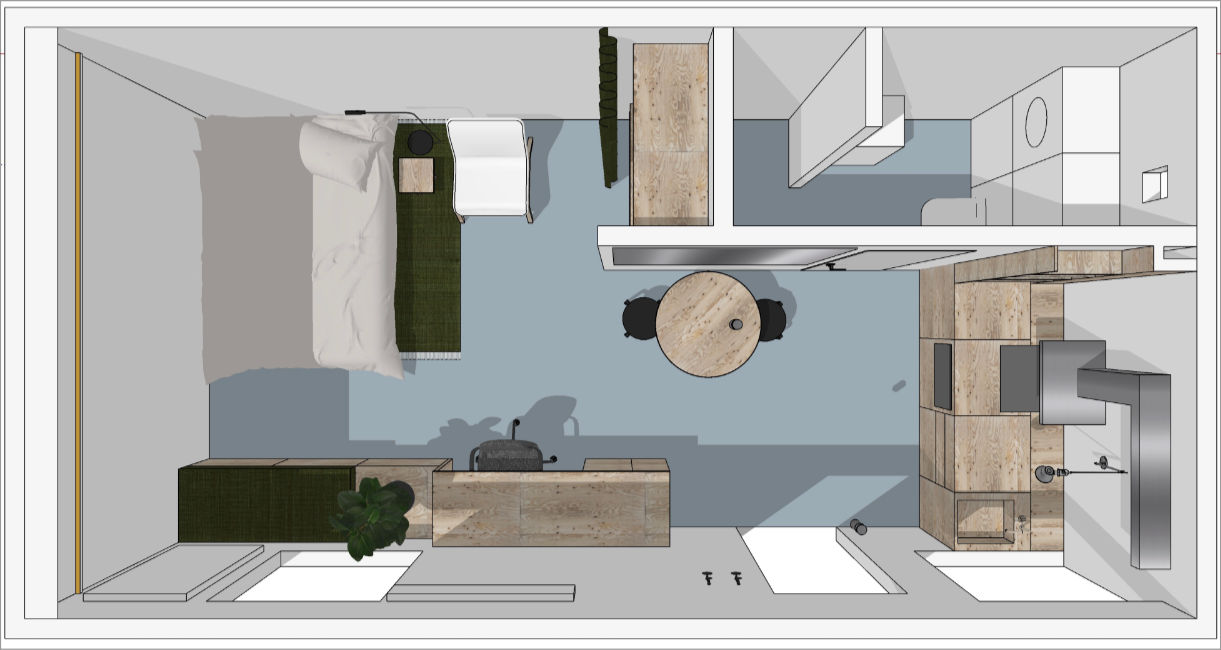
\includegraphics[width=.9\linewidth]{Приложение/2025-03-19_12-29-29_screenshot.png}
\end{center}

\href{https://drive.google.com/file/d/13h-R1aoj9f6Z40jsrrGZrNA3UMwl2f0N/view?usp=sharing}{Исходный файл SketchUp}
\end{document}
